% Options for packages loaded elsewhere
\PassOptionsToPackage{unicode}{hyperref}
\PassOptionsToPackage{hyphens}{url}
\PassOptionsToPackage{dvipsnames,svgnames,x11names}{xcolor}
%
\documentclass[
  letterpaper,
  DIV=11,
  numbers=noendperiod]{scrartcl}

\usepackage{amsmath,amssymb}
\usepackage{iftex}
\ifPDFTeX
  \usepackage[T1]{fontenc}
  \usepackage[utf8]{inputenc}
  \usepackage{textcomp} % provide euro and other symbols
\else % if luatex or xetex
  \usepackage{unicode-math}
  \defaultfontfeatures{Scale=MatchLowercase}
  \defaultfontfeatures[\rmfamily]{Ligatures=TeX,Scale=1}
\fi
\usepackage{lmodern}
\ifPDFTeX\else  
    % xetex/luatex font selection
\fi
% Use upquote if available, for straight quotes in verbatim environments
\IfFileExists{upquote.sty}{\usepackage{upquote}}{}
\IfFileExists{microtype.sty}{% use microtype if available
  \usepackage[]{microtype}
  \UseMicrotypeSet[protrusion]{basicmath} % disable protrusion for tt fonts
}{}
\makeatletter
\@ifundefined{KOMAClassName}{% if non-KOMA class
  \IfFileExists{parskip.sty}{%
    \usepackage{parskip}
  }{% else
    \setlength{\parindent}{0pt}
    \setlength{\parskip}{6pt plus 2pt minus 1pt}}
}{% if KOMA class
  \KOMAoptions{parskip=half}}
\makeatother
\usepackage{xcolor}
\setlength{\emergencystretch}{3em} % prevent overfull lines
\setcounter{secnumdepth}{-\maxdimen} % remove section numbering
% Make \paragraph and \subparagraph free-standing
\makeatletter
\ifx\paragraph\undefined\else
  \let\oldparagraph\paragraph
  \renewcommand{\paragraph}{
    \@ifstar
      \xxxParagraphStar
      \xxxParagraphNoStar
  }
  \newcommand{\xxxParagraphStar}[1]{\oldparagraph*{#1}\mbox{}}
  \newcommand{\xxxParagraphNoStar}[1]{\oldparagraph{#1}\mbox{}}
\fi
\ifx\subparagraph\undefined\else
  \let\oldsubparagraph\subparagraph
  \renewcommand{\subparagraph}{
    \@ifstar
      \xxxSubParagraphStar
      \xxxSubParagraphNoStar
  }
  \newcommand{\xxxSubParagraphStar}[1]{\oldsubparagraph*{#1}\mbox{}}
  \newcommand{\xxxSubParagraphNoStar}[1]{\oldsubparagraph{#1}\mbox{}}
\fi
\makeatother

\usepackage{color}
\usepackage{fancyvrb}
\newcommand{\VerbBar}{|}
\newcommand{\VERB}{\Verb[commandchars=\\\{\}]}
\DefineVerbatimEnvironment{Highlighting}{Verbatim}{commandchars=\\\{\}}
% Add ',fontsize=\small' for more characters per line
\usepackage{framed}
\definecolor{shadecolor}{RGB}{241,243,245}
\newenvironment{Shaded}{\begin{snugshade}}{\end{snugshade}}
\newcommand{\AlertTok}[1]{\textcolor[rgb]{0.68,0.00,0.00}{#1}}
\newcommand{\AnnotationTok}[1]{\textcolor[rgb]{0.37,0.37,0.37}{#1}}
\newcommand{\AttributeTok}[1]{\textcolor[rgb]{0.40,0.45,0.13}{#1}}
\newcommand{\BaseNTok}[1]{\textcolor[rgb]{0.68,0.00,0.00}{#1}}
\newcommand{\BuiltInTok}[1]{\textcolor[rgb]{0.00,0.23,0.31}{#1}}
\newcommand{\CharTok}[1]{\textcolor[rgb]{0.13,0.47,0.30}{#1}}
\newcommand{\CommentTok}[1]{\textcolor[rgb]{0.37,0.37,0.37}{#1}}
\newcommand{\CommentVarTok}[1]{\textcolor[rgb]{0.37,0.37,0.37}{\textit{#1}}}
\newcommand{\ConstantTok}[1]{\textcolor[rgb]{0.56,0.35,0.01}{#1}}
\newcommand{\ControlFlowTok}[1]{\textcolor[rgb]{0.00,0.23,0.31}{\textbf{#1}}}
\newcommand{\DataTypeTok}[1]{\textcolor[rgb]{0.68,0.00,0.00}{#1}}
\newcommand{\DecValTok}[1]{\textcolor[rgb]{0.68,0.00,0.00}{#1}}
\newcommand{\DocumentationTok}[1]{\textcolor[rgb]{0.37,0.37,0.37}{\textit{#1}}}
\newcommand{\ErrorTok}[1]{\textcolor[rgb]{0.68,0.00,0.00}{#1}}
\newcommand{\ExtensionTok}[1]{\textcolor[rgb]{0.00,0.23,0.31}{#1}}
\newcommand{\FloatTok}[1]{\textcolor[rgb]{0.68,0.00,0.00}{#1}}
\newcommand{\FunctionTok}[1]{\textcolor[rgb]{0.28,0.35,0.67}{#1}}
\newcommand{\ImportTok}[1]{\textcolor[rgb]{0.00,0.46,0.62}{#1}}
\newcommand{\InformationTok}[1]{\textcolor[rgb]{0.37,0.37,0.37}{#1}}
\newcommand{\KeywordTok}[1]{\textcolor[rgb]{0.00,0.23,0.31}{\textbf{#1}}}
\newcommand{\NormalTok}[1]{\textcolor[rgb]{0.00,0.23,0.31}{#1}}
\newcommand{\OperatorTok}[1]{\textcolor[rgb]{0.37,0.37,0.37}{#1}}
\newcommand{\OtherTok}[1]{\textcolor[rgb]{0.00,0.23,0.31}{#1}}
\newcommand{\PreprocessorTok}[1]{\textcolor[rgb]{0.68,0.00,0.00}{#1}}
\newcommand{\RegionMarkerTok}[1]{\textcolor[rgb]{0.00,0.23,0.31}{#1}}
\newcommand{\SpecialCharTok}[1]{\textcolor[rgb]{0.37,0.37,0.37}{#1}}
\newcommand{\SpecialStringTok}[1]{\textcolor[rgb]{0.13,0.47,0.30}{#1}}
\newcommand{\StringTok}[1]{\textcolor[rgb]{0.13,0.47,0.30}{#1}}
\newcommand{\VariableTok}[1]{\textcolor[rgb]{0.07,0.07,0.07}{#1}}
\newcommand{\VerbatimStringTok}[1]{\textcolor[rgb]{0.13,0.47,0.30}{#1}}
\newcommand{\WarningTok}[1]{\textcolor[rgb]{0.37,0.37,0.37}{\textit{#1}}}

\providecommand{\tightlist}{%
  \setlength{\itemsep}{0pt}\setlength{\parskip}{0pt}}\usepackage{longtable,booktabs,array}
\usepackage{calc} % for calculating minipage widths
% Correct order of tables after \paragraph or \subparagraph
\usepackage{etoolbox}
\makeatletter
\patchcmd\longtable{\par}{\if@noskipsec\mbox{}\fi\par}{}{}
\makeatother
% Allow footnotes in longtable head/foot
\IfFileExists{footnotehyper.sty}{\usepackage{footnotehyper}}{\usepackage{footnote}}
\makesavenoteenv{longtable}
\usepackage{graphicx}
\makeatletter
\newsavebox\pandoc@box
\newcommand*\pandocbounded[1]{% scales image to fit in text height/width
  \sbox\pandoc@box{#1}%
  \Gscale@div\@tempa{\textheight}{\dimexpr\ht\pandoc@box+\dp\pandoc@box\relax}%
  \Gscale@div\@tempb{\linewidth}{\wd\pandoc@box}%
  \ifdim\@tempb\p@<\@tempa\p@\let\@tempa\@tempb\fi% select the smaller of both
  \ifdim\@tempa\p@<\p@\scalebox{\@tempa}{\usebox\pandoc@box}%
  \else\usebox{\pandoc@box}%
  \fi%
}
% Set default figure placement to htbp
\def\fps@figure{htbp}
\makeatother

\KOMAoption{captions}{tableheading}
\makeatletter
\@ifpackageloaded{caption}{}{\usepackage{caption}}
\AtBeginDocument{%
\ifdefined\contentsname
  \renewcommand*\contentsname{Table of contents}
\else
  \newcommand\contentsname{Table of contents}
\fi
\ifdefined\listfigurename
  \renewcommand*\listfigurename{List of Figures}
\else
  \newcommand\listfigurename{List of Figures}
\fi
\ifdefined\listtablename
  \renewcommand*\listtablename{List of Tables}
\else
  \newcommand\listtablename{List of Tables}
\fi
\ifdefined\figurename
  \renewcommand*\figurename{Figure}
\else
  \newcommand\figurename{Figure}
\fi
\ifdefined\tablename
  \renewcommand*\tablename{Table}
\else
  \newcommand\tablename{Table}
\fi
}
\@ifpackageloaded{float}{}{\usepackage{float}}
\floatstyle{ruled}
\@ifundefined{c@chapter}{\newfloat{codelisting}{h}{lop}}{\newfloat{codelisting}{h}{lop}[chapter]}
\floatname{codelisting}{Listing}
\newcommand*\listoflistings{\listof{codelisting}{List of Listings}}
\makeatother
\makeatletter
\makeatother
\makeatletter
\@ifpackageloaded{caption}{}{\usepackage{caption}}
\@ifpackageloaded{subcaption}{}{\usepackage{subcaption}}
\makeatother

\usepackage{bookmark}

\IfFileExists{xurl.sty}{\usepackage{xurl}}{} % add URL line breaks if available
\urlstyle{same} % disable monospaced font for URLs
\hypersetup{
  pdftitle={exer},
  pdfauthor={yoon},
  colorlinks=true,
  linkcolor={blue},
  filecolor={Maroon},
  citecolor={Blue},
  urlcolor={Blue},
  pdfcreator={LaTeX via pandoc}}


\title{exer}
\author{yoon}
\date{}

\begin{document}
\maketitle


\section{기말 연습용}\label{uxae30uxb9d0-uxc5f0uxc2b5uxc6a9}

\subsection{1. 선형을 활용한
예측}\label{uxc120uxd615uxc744-uxd65cuxc6a9uxd55c-uxc608uxce21}

\subsubsection{1-1. loading}\label{loading}

\begin{Shaded}
\begin{Highlighting}[]
\FunctionTok{library}\NormalTok{(caret)}
\end{Highlighting}
\end{Shaded}

\begin{verbatim}
Loading required package: ggplot2
\end{verbatim}

\begin{verbatim}
Loading required package: lattice
\end{verbatim}

\begin{Shaded}
\begin{Highlighting}[]
\FunctionTok{library}\NormalTok{(MASS)}
\FunctionTok{library}\NormalTok{(tidyverse)}
\end{Highlighting}
\end{Shaded}

\begin{verbatim}
-- Attaching core tidyverse packages ------------------------ tidyverse 2.0.0 --
v dplyr     1.1.4     v readr     2.1.4
v forcats   1.0.0     v stringr   1.5.1
v lubridate 1.9.3     v tibble    3.2.1
v purrr     1.0.2     v tidyr     1.3.0
\end{verbatim}

\begin{verbatim}
-- Conflicts ------------------------------------------ tidyverse_conflicts() --
x dplyr::filter() masks stats::filter()
x dplyr::lag()    masks stats::lag()
x purrr::lift()   masks caret::lift()
x dplyr::select() masks MASS::select()
i Use the conflicted package (<http://conflicted.r-lib.org/>) to force all conflicts to become errors
\end{verbatim}

\begin{Shaded}
\begin{Highlighting}[]
\NormalTok{gpa }\OtherTok{\textless{}{-}} \FunctionTok{read.csv}\NormalTok{(}\StringTok{"dataforclass/gpa1.csv"}\NormalTok{,}\AttributeTok{header =} \ConstantTok{TRUE}\NormalTok{,}
                \AttributeTok{sep =} \StringTok{"}\SpecialCharTok{\textbackslash{}t}\StringTok{"}\NormalTok{)}
\FunctionTok{str}\NormalTok{(gpa)}
\end{Highlighting}
\end{Shaded}

\begin{verbatim}
'data.frame':   141 obs. of  29 variables:
 $ age     : int  21 21 20 19 20 20 22 22 22 19 ...
 $ soph    : int  0 0 0 1 0 0 0 0 0 1 ...
 $ junior  : int  0 0 1 0 1 0 0 0 0 0 ...
 $ senior  : int  1 1 0 0 0 1 0 0 0 0 ...
 $ senior5 : int  0 0 0 0 0 0 1 1 1 0 ...
 $ male    : int  0 0 0 1 0 1 0 0 0 0 ...
 $ campus  : int  0 0 0 1 0 1 0 0 0 0 ...
 $ business: int  1 1 1 1 1 1 1 0 0 1 ...
 $ engineer: int  0 0 0 0 0 0 0 0 0 0 ...
 $ colGPA  : num  3 3.4 3 3.5 3.6 ...
 $ hsGPA   : num  3 3.2 3.6 3.5 3.9 ...
 $ ACT     : int  21 24 26 27 28 25 25 22 21 27 ...
 $ job19   : int  0 0 1 1 0 0 0 1 1 1 ...
 $ job20   : int  1 1 0 0 1 0 0 0 0 0 ...
 $ drive   : int  1 1 0 0 0 0 0 1 1 0 ...
 $ bike    : int  0 0 0 0 1 0 1 0 0 0 ...
 $ walk    : int  0 0 1 1 0 1 0 0 0 1 ...
 $ voluntr : int  0 0 0 0 0 0 0 0 0 0 ...
 $ PC      : int  0 0 0 0 0 0 0 1 0 1 ...
 $ greek   : int  0 0 0 0 0 0 1 0 0 0 ...
 $ car     : int  1 1 1 0 1 1 1 0 1 0 ...
 $ siblings: int  1 0 1 1 1 1 1 1 1 1 ...
 $ bgfriend: int  0 1 0 0 1 0 0 1 1 0 ...
 $ clubs   : int  0 1 1 0 0 0 1 0 1 1 ...
 $ skipped : num  2 0 0 0 0 0 0 3 2 0.5 ...
 $ alcohol : num  1 1 1 0 1.5 0 2 3 2.5 0.75 ...
 $ gradMI  : int  1 1 1 0 1 0 1 1 1 1 ...
 $ fathcoll: int  0 1 1 0 1 1 0 1 1 0 ...
 $ mothcoll: int  0 1 1 0 0 0 1 1 1 1 ...
\end{verbatim}

\subsubsection{1-2. train과 test 데이터
구분}\label{trainuxacfc-test-uxb370uxc774uxd130-uxad6cuxbd84}

\begin{itemize}
\tightlist
\item
  데이터 구분
\end{itemize}

\begin{Shaded}
\begin{Highlighting}[]
\NormalTok{train\_i }\OtherTok{\textless{}{-}} \FunctionTok{createDataPartition}\NormalTok{(gpa}\SpecialCharTok{$}\NormalTok{colGPA,}
                               \AttributeTok{p =} \FloatTok{0.8}\NormalTok{,}
                               \AttributeTok{list =} \ConstantTok{FALSE}\NormalTok{) }
\NormalTok{train }\OtherTok{\textless{}{-}}\NormalTok{ gpa[train\_i,]}
\NormalTok{test }\OtherTok{\textless{}{-}}\NormalTok{ gpa[}\SpecialCharTok{{-}}\NormalTok{train\_i,]}
\FunctionTok{str}\NormalTok{(train)}
\end{Highlighting}
\end{Shaded}

\begin{verbatim}
'data.frame':   115 obs. of  29 variables:
 $ age     : int  21 21 20 19 20 20 22 22 22 19 ...
 $ soph    : int  0 0 0 1 0 0 0 0 0 1 ...
 $ junior  : int  0 0 1 0 1 0 0 0 0 0 ...
 $ senior  : int  1 1 0 0 0 1 0 0 0 0 ...
 $ senior5 : int  0 0 0 0 0 0 1 1 1 0 ...
 $ male    : int  0 0 0 1 0 1 0 0 0 0 ...
 $ campus  : int  0 0 0 1 0 1 0 0 0 0 ...
 $ business: int  1 1 1 1 1 1 1 0 0 1 ...
 $ engineer: int  0 0 0 0 0 0 0 0 0 0 ...
 $ colGPA  : num  3 3.4 3 3.5 3.6 ...
 $ hsGPA   : num  3 3.2 3.6 3.5 3.9 ...
 $ ACT     : int  21 24 26 27 28 25 25 22 21 27 ...
 $ job19   : int  0 0 1 1 0 0 0 1 1 1 ...
 $ job20   : int  1 1 0 0 1 0 0 0 0 0 ...
 $ drive   : int  1 1 0 0 0 0 0 1 1 0 ...
 $ bike    : int  0 0 0 0 1 0 1 0 0 0 ...
 $ walk    : int  0 0 1 1 0 1 0 0 0 1 ...
 $ voluntr : int  0 0 0 0 0 0 0 0 0 0 ...
 $ PC      : int  0 0 0 0 0 0 0 1 0 1 ...
 $ greek   : int  0 0 0 0 0 0 1 0 0 0 ...
 $ car     : int  1 1 1 0 1 1 1 0 1 0 ...
 $ siblings: int  1 0 1 1 1 1 1 1 1 1 ...
 $ bgfriend: int  0 1 0 0 1 0 0 1 1 0 ...
 $ clubs   : int  0 1 1 0 0 0 1 0 1 1 ...
 $ skipped : num  2 0 0 0 0 0 0 3 2 0.5 ...
 $ alcohol : num  1 1 1 0 1.5 0 2 3 2.5 0.75 ...
 $ gradMI  : int  1 1 1 0 1 0 1 1 1 1 ...
 $ fathcoll: int  0 1 1 0 1 1 0 1 1 0 ...
 $ mothcoll: int  0 1 1 0 0 0 1 1 1 1 ...
\end{verbatim}

\begin{Shaded}
\begin{Highlighting}[]
\FunctionTok{str}\NormalTok{(test)}
\end{Highlighting}
\end{Shaded}

\begin{verbatim}
'data.frame':   26 obs. of  29 variables:
 $ age     : int  20 20 20 21 22 21 19 20 22 21 ...
 $ soph    : int  0 0 0 0 0 0 0 0 0 0 ...
 $ junior  : int  1 1 1 0 0 0 1 0 0 0 ...
 $ senior  : int  0 0 0 1 1 1 0 1 0 1 ...
 $ senior5 : int  0 0 0 0 0 0 0 0 1 0 ...
 $ male    : int  0 1 0 0 1 1 0 1 1 1 ...
 $ campus  : int  0 0 0 0 0 0 0 1 0 0 ...
 $ business: int  1 1 1 1 1 1 1 0 1 0 ...
 $ engineer: int  0 0 0 0 0 0 0 1 0 0 ...
 $ colGPA  : num  2.9 3.3 3.4 3.5 3.7 ...
 $ hsGPA   : num  3.6 3.6 3.7 3.3 3.3 ...
 $ ACT     : int  27 33 24 23 22 23 21 19 27 27 ...
 $ job19   : int  0 0 0 0 0 0 1 1 0 1 ...
 $ job20   : int  0 0 0 0 0 1 0 0 0 0 ...
 $ drive   : int  0 0 0 1 0 0 0 0 1 0 ...
 $ bike    : int  1 1 1 0 1 0 0 1 0 0 ...
 $ walk    : int  0 0 0 0 0 1 1 0 0 1 ...
 $ voluntr : int  1 1 0 0 0 1 1 1 0 0 ...
 $ PC      : int  1 0 0 1 1 1 0 1 0 0 ...
 $ greek   : int  0 1 1 1 0 1 0 0 0 0 ...
 $ car     : int  1 0 0 1 1 0 1 1 1 1 ...
 $ siblings: int  1 1 1 1 1 1 1 1 1 1 ...
 $ bgfriend: int  1 1 1 1 1 0 0 0 0 0 ...
 $ clubs   : int  1 0 0 0 1 1 1 1 0 1 ...
 $ skipped : num  1 2 0.5 1 0 0 0 1 2 0 ...
 $ alcohol : num  1 5 2 0 1 2 2 0 5 1 ...
 $ gradMI  : int  0 1 1 1 1 1 1 1 1 1 ...
 $ fathcoll: int  1 1 1 1 1 1 1 1 1 1 ...
 $ mothcoll: int  0 0 1 1 0 1 1 0 1 1 ...
\end{verbatim}

\subsubsection{1-3. 선형모형 제작과 예측
실험}\label{uxc120uxd615uxbaa8uxd615-uxc81cuxc791uxacfc-uxc608uxce21-uxc2e4uxd5d8}

\begin{itemize}
\tightlist
\item
  선형 모델 제작
\end{itemize}

\begin{Shaded}
\begin{Highlighting}[]
\NormalTok{lm\_gpa }\OtherTok{\textless{}{-}} \FunctionTok{lm}\NormalTok{(colGPA}\SpecialCharTok{\textasciitilde{}}\NormalTok{., }\AttributeTok{data =}\NormalTok{ train)}
\FunctionTok{summary}\NormalTok{(lm\_gpa)}
\end{Highlighting}
\end{Shaded}

\begin{verbatim}

Call:
lm(formula = colGPA ~ ., data = train)

Residuals:
     Min       1Q   Median       3Q      Max 
-0.63106 -0.19232 -0.01799  0.20445  0.67404 

Coefficients: (2 not defined because of singularities)
              Estimate Std. Error t value Pr(>|t|)    
(Intercept)  8.124e-01  8.540e-01   0.951  0.34402    
age          1.066e-02  3.206e-02   0.332  0.74036    
soph         1.683e-01  2.593e-01   0.649  0.51792    
junior      -1.997e-03  1.392e-01  -0.014  0.98858    
senior      -1.207e-02  1.235e-01  -0.098  0.92236    
senior5             NA         NA      NA       NA    
male         1.326e-01  7.803e-02   1.700  0.09271 .  
campus      -1.911e-01  9.503e-02  -2.011  0.04734 *  
business     1.429e-02  9.511e-02   0.150  0.88093    
engineer    -2.715e-01  2.101e-01  -1.292  0.19980    
hsGPA        5.292e-01  1.123e-01   4.712 9.12e-06 ***
ACT          6.950e-03  1.276e-02   0.545  0.58738    
job19        3.959e-02  7.107e-02   0.557  0.57888    
job20        1.282e-01  9.701e-02   1.322  0.18959    
drive       -1.683e-03  9.657e-02  -0.017  0.98613    
bike        -7.468e-02  7.576e-02  -0.986  0.32694    
walk                NA         NA      NA       NA    
voluntr      1.211e-02  8.590e-02   0.141  0.88819    
PC           1.193e-01  6.924e-02   1.723  0.08835 .  
greek        6.721e-02  7.246e-02   0.928  0.35620    
car         -4.580e-02  8.349e-02  -0.549  0.58472    
siblings    -1.144e-01  1.350e-01  -0.847  0.39921    
bgfriend     2.163e-02  6.510e-02   0.332  0.74055    
clubs        5.243e-02  6.606e-02   0.794  0.42952    
skipped     -1.037e-01  3.353e-02  -3.094  0.00265 ** 
alcohol     -5.349e-05  2.979e-02  -0.002  0.99857    
gradMI       2.025e-01  1.016e-01   1.993  0.04931 *  
fathcoll     2.174e-02  7.185e-02   0.303  0.76297    
mothcoll    -4.858e-02  8.106e-02  -0.599  0.55053    
---
Signif. codes:  0 '***' 0.001 '**' 0.01 '*' 0.05 '.' 0.1 ' ' 1

Residual standard error: 0.3119 on 88 degrees of freedom
Multiple R-squared:  0.4577,    Adjusted R-squared:  0.2975 
F-statistic: 2.857 on 26 and 88 DF,  p-value: 0.0001368
\end{verbatim}

\begin{itemize}
\tightlist
\item
  예측값 계산
\end{itemize}

\begin{Shaded}
\begin{Highlighting}[]
\NormalTok{predic\_gpa }\OtherTok{\textless{}{-}} \FunctionTok{predict}\NormalTok{(lm\_gpa,}\AttributeTok{newdata =}\NormalTok{ test)}

\NormalTok{result }\OtherTok{\textless{}{-}} \FunctionTok{data.frame}\NormalTok{(}
  \AttributeTok{actual =}\NormalTok{ test}\SpecialCharTok{$}\NormalTok{colGPA,}
  \AttributeTok{predict =}\NormalTok{ predic\_gpa}
\NormalTok{)}
\FunctionTok{head}\NormalTok{(result)}
\end{Highlighting}
\end{Shaded}

\begin{verbatim}
   actual  predict
23    2.9 3.019296
25    3.3 3.233469
30    3.4 3.186287
32    3.5 3.062993
33    3.7 3.263808
42    2.8 3.729574
\end{verbatim}

\begin{itemize}
\tightlist
\item
  예측값 시각화
\end{itemize}

\begin{Shaded}
\begin{Highlighting}[]
\NormalTok{result }\SpecialCharTok{|\textgreater{}} 
  \FunctionTok{ggplot}\NormalTok{(}\AttributeTok{mapping =} \FunctionTok{aes}\NormalTok{(}\AttributeTok{x =}\NormalTok{ actual, }\AttributeTok{y =}\NormalTok{ predict)) }\SpecialCharTok{+} 
  \FunctionTok{geom\_point}\NormalTok{() }\SpecialCharTok{+} 
  \FunctionTok{geom\_abline}\NormalTok{(}\AttributeTok{intercept =} \DecValTok{0}\NormalTok{ , }\AttributeTok{slope =} \DecValTok{1}\NormalTok{, }\AttributeTok{color =} \StringTok{"red"}\NormalTok{, }\AttributeTok{linetype =} \StringTok{"dashed"}\NormalTok{)}
\end{Highlighting}
\end{Shaded}

\pandocbounded{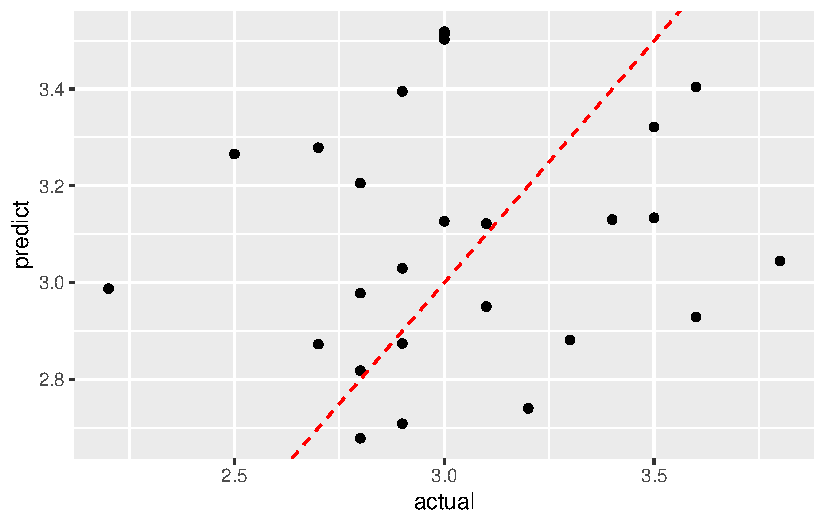
\includegraphics[keepaspectratio]{exer_files/figure-pdf/unnamed-chunk-6-1.pdf}}

\begin{Shaded}
\begin{Highlighting}[]
  \FunctionTok{labs}\NormalTok{( }
    \AttributeTok{x =} \StringTok{"실제 GPA"}\NormalTok{, }\AttributeTok{y =} \StringTok{"예측 GPA"}
\NormalTok{    )}
\end{Highlighting}
\end{Shaded}

\begin{verbatim}
$x
[1] "실제 GPA"

$y
[1] "예측 GPA"

attr(,"class")
[1] "labels"
\end{verbatim}

\begin{itemize}
\tightlist
\item
  MSE 와 RMSE
\end{itemize}

\begin{Shaded}
\begin{Highlighting}[]
\CommentTok{\# 계산}
\NormalTok{mse }\OtherTok{=} \FunctionTok{mean}\NormalTok{(result}\SpecialCharTok{$}\NormalTok{actual }\SpecialCharTok{{-}}\NormalTok{ result}\SpecialCharTok{$}\NormalTok{predict)}\SpecialCharTok{\^{}}\DecValTok{2}
\NormalTok{rmse }\OtherTok{=} \FunctionTok{sqrt}\NormalTok{(mse)}

\CommentTok{\# 값 확인 }
\FunctionTok{print}\NormalTok{(}\FunctionTok{paste}\NormalTok{(}\StringTok{"MSE = "}\NormalTok{, mse))}
\end{Highlighting}
\end{Shaded}

\begin{verbatim}
[1] "MSE =  0.00697309703425082"
\end{verbatim}

\begin{Shaded}
\begin{Highlighting}[]
\FunctionTok{print}\NormalTok{(}\FunctionTok{paste}\NormalTok{(}\StringTok{"RMSE = "}\NormalTok{, rmse))}
\end{Highlighting}
\end{Shaded}

\begin{verbatim}
[1] "RMSE =  0.0835050719073447"
\end{verbatim}

\subsubsection{1-4. 모델 선택}\label{uxbaa8uxb378-uxc120uxd0dd}

\begin{itemize}
\tightlist
\item
  AIC 방법을 활용한 모델 선택
\end{itemize}

\begin{Shaded}
\begin{Highlighting}[]
\CommentTok{\# 모델 확인 }
\NormalTok{slected\_model }\OtherTok{\textless{}{-}}  \FunctionTok{stepAIC}\NormalTok{(}\FunctionTok{lm}\NormalTok{(colGPA }\SpecialCharTok{\textasciitilde{}}\NormalTok{.,}\AttributeTok{data =}\NormalTok{ train),}
                          \AttributeTok{direction =} \StringTok{"both"}\NormalTok{,}
                          \AttributeTok{trace =} \ConstantTok{FALSE}
\NormalTok{                          )}

\CommentTok{\# 선택된 모델 확인}
\NormalTok{model }\OtherTok{\textless{}{-}} \FunctionTok{names}\NormalTok{(}\FunctionTok{coef}\NormalTok{(slected\_model))[}\SpecialCharTok{{-}}\DecValTok{1}\NormalTok{]}
\FunctionTok{print}\NormalTok{(model)}
\end{Highlighting}
\end{Shaded}

\begin{verbatim}
[1] "male"     "campus"   "engineer" "hsGPA"    "job20"    "PC"       "skipped" 
[8] "gradMI"  
\end{verbatim}

\begin{Shaded}
\begin{Highlighting}[]
\CommentTok{\# 모델 붙여넣기 }
\NormalTok{temp }\OtherTok{\textless{}{-}} \FunctionTok{paste}\NormalTok{(model, }\AttributeTok{collapse =} \StringTok{" + "}\NormalTok{)}
\NormalTok{formula }\OtherTok{\textless{}{-}}\FunctionTok{as.formula}\NormalTok{(}\FunctionTok{paste}\NormalTok{(}\StringTok{"colGPA \textasciitilde{}"}\NormalTok{,temp))}

\NormalTok{lm\_selected }\OtherTok{\textless{}{-}} \FunctionTok{lm}\NormalTok{(formula, }\AttributeTok{data =}\NormalTok{ train)}
\FunctionTok{summary}\NormalTok{(lm\_selected)}
\end{Highlighting}
\end{Shaded}

\begin{verbatim}

Call:
lm(formula = formula, data = train)

Residuals:
     Min       1Q   Median       3Q      Max 
-0.57853 -0.22377 -0.00639  0.21142  0.65313 

Coefficients:
            Estimate Std. Error t value Pr(>|t|)    
(Intercept)  1.02607    0.31617   3.245 0.001571 ** 
male         0.11935    0.05921   2.016 0.046366 *  
campus      -0.17328    0.08118  -2.134 0.035107 *  
engineer    -0.26468    0.15862  -1.669 0.098141 .  
hsGPA        0.55414    0.08658   6.400 4.31e-09 ***
job20        0.12304    0.07780   1.581 0.116752    
PC           0.14398    0.05915   2.434 0.016606 *  
skipped     -0.09064    0.02644  -3.428 0.000866 ***
gradMI       0.17984    0.08466   2.124 0.035974 *  
---
Signif. codes:  0 '***' 0.001 '**' 0.01 '*' 0.05 '.' 0.1 ' ' 1

Residual standard error: 0.2928 on 106 degrees of freedom
Multiple R-squared:  0.4244,    Adjusted R-squared:  0.3809 
F-statistic: 9.767 on 8 and 106 DF,  p-value: 4.441e-10
\end{verbatim}




\end{document}
